\documentclass[12pt]{article}
\usepackage{graphicx}
%\usepackage{amsmath}
\usepackage{amsmath}
\usepackage{amssymb}
\usepackage{tikz}
\title{C-Space of a 2-link Planar Manipulator Arm}
\date{}
\begin{document}
\maketitle
\section*{Introduction}
In robotic motion planning, the workspace is the physical environment containing the robot and obstacles, while the configuration space (C-space) represents all possible joint configurations. Each point in C-space corresponds to a unique robot pose, and the mapping from workspace to C-space becomes highly non-linear when obstacles are present. We begin by exploring a discretized angle-based method that generates binary collision maps for various obstacle positions. To overcome the limitations of this approach, we later adopt a geometric method that starts by identifying safe angular ranges for the first link of a 2R manipulator, and then extends to the second link for interpretable collision avoidance.

\section{Binary Matrices Approach}
In this method, we start with a simple 2R planar manipulator, which is kept near a small rectangular obstacle. The goal of this process is to find the set of joint angles of the robot, for which there is a collision-free motion. We are tasked with mapping the C-Space from the given workspace. For this, we use MATLAB R2024b. We start off by discretizing the values of both the joint angles, in steps of 2 degrees. Let us denote first joint angle as $\theta_1$, and the second joint angle measured with respect to the first link, as $\theta_2$. So now, we have both these angles taking values such as 0, 2, 4, ....upto 360 degrees. We assume there are no joint limits for this analysis.
\newline
We can observe that each unique configuration of the robot needs 2 parameters, which are basically $\theta_1$ and $\theta_2$. Since we discretize in steps of 2 degrees, both $\theta_1$ and $\theta_2$ can take 181 different angle values, starting from 0 and going till 360 degrees. So there are 181 x 181 unique configurations of the robot that is possible for the chosen discretization. We put all of these 181 x 181 values inside a square matrix having 181 rows and 181 columns. Also, there will be some configurations of the robot which will collide with the obstacle, while others may not. For all the configurations that collide with some part of the obstacle, we assign a value of 1 in the corresponding position of the 181 x 181 matrix. Collision free positions are denoted by 0 in the matrix. Now we finally have a matrix that contains only zeros and ones. We call this the binary matrix which tells us which configurations are collision free, and those which are collision prone.
\newline
We shall now get a visual idea of the C-Space by plotting the binary matrix. Create a plot with X-Axis as $\theta_1$ and Y-Axis as $\theta_2$. Use the binary matrix values to construct the plot. The collision prone configurations of the robot will be denoted by the number 1 in the matrix; so while plotting these, we assign black colour. Collision free configurations need not be plotted explicitly in any colour, as we are already plotting the collision prone positions in black. After plotting completely, we can get a plot which is shaded black in some regions, and others regions are just plain. The black regions correspond to all the collision-prone configurations, while the plain regions are collision-free configurations.
\begin{figure}[h]
    \centering
    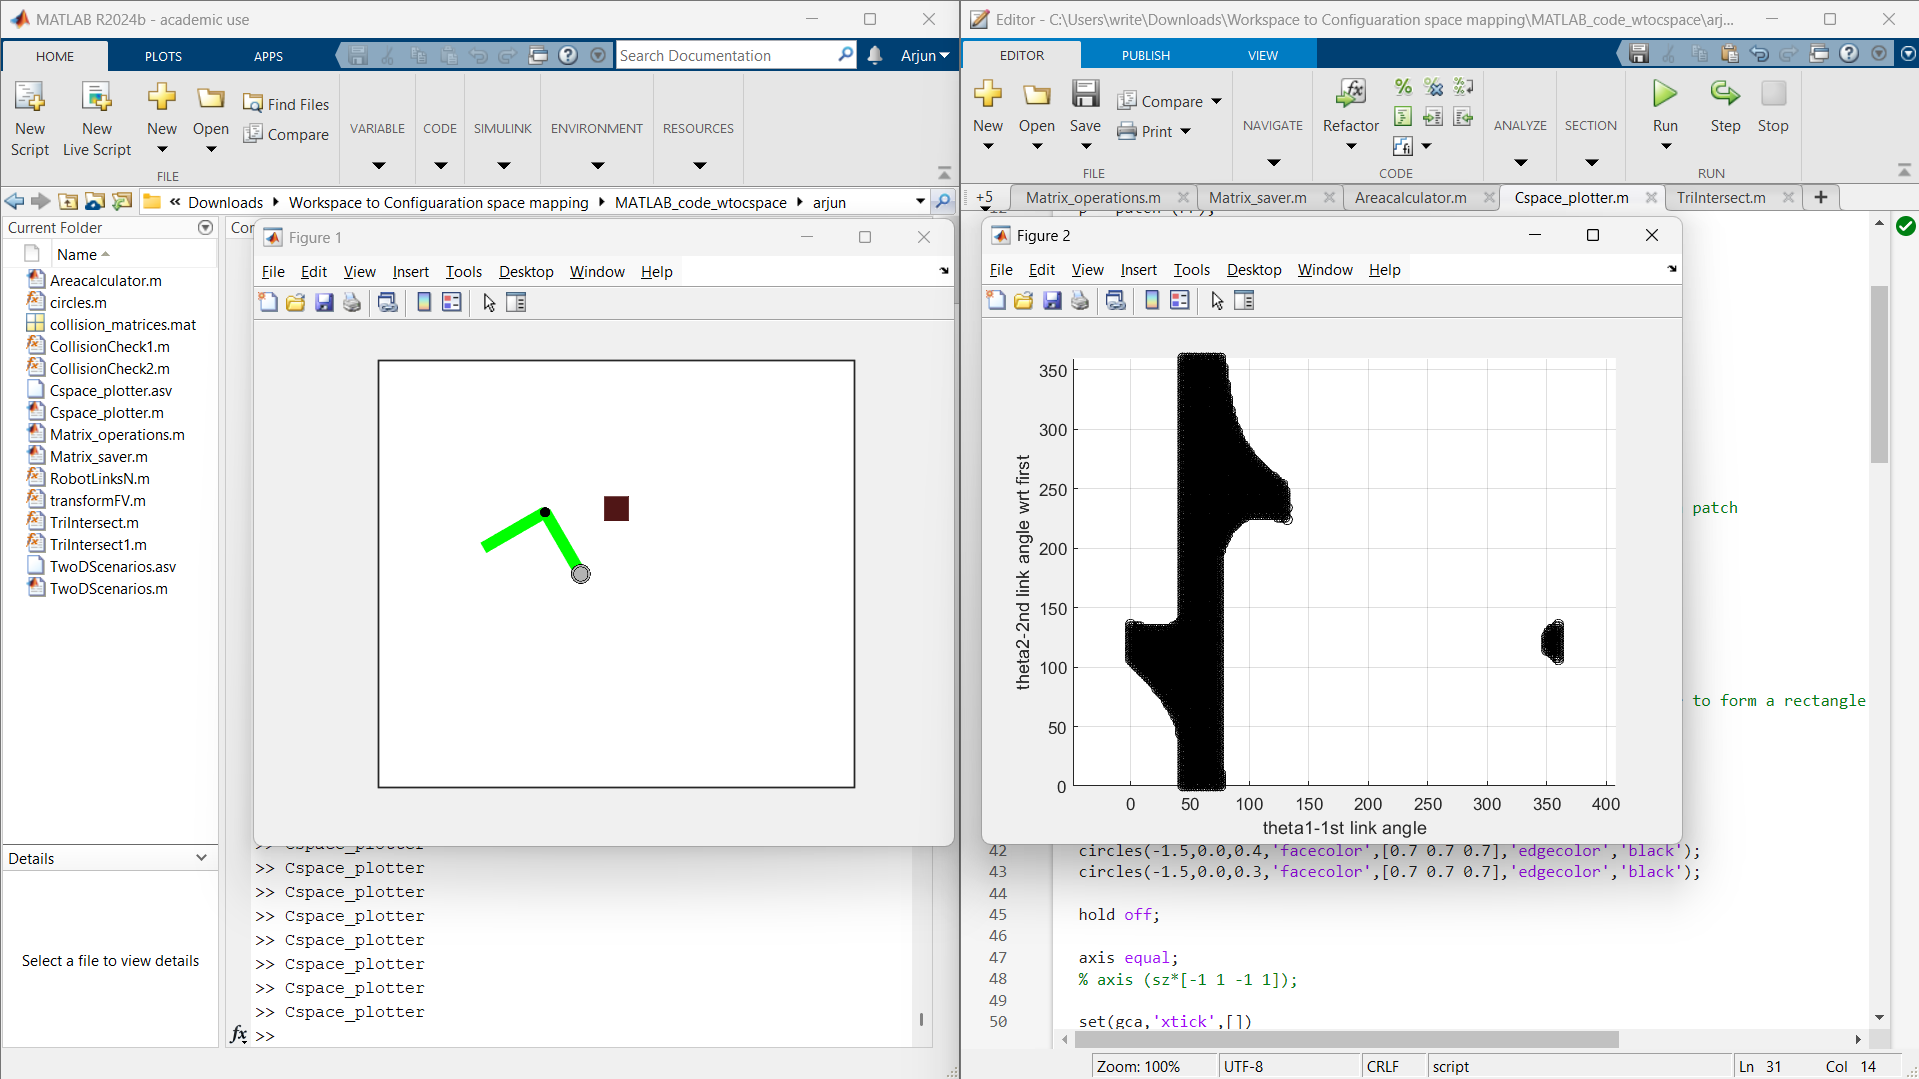
\includegraphics[width=1.0\textwidth]{Screenshot 2025-05-15 115430}
    \caption{Window on the right shows the plot between $\theta_2$ and $\theta_1$}
    \label{fig:1}
\end{figure}
\newline
Next, we try to observe the variation in the C-Space plot, for a given input motion of the obstacle. We start off by considering a simple unidirectional translation of the obstacle along the vertical direction; and we plot the C-Space by sampling different positions that the obstacle would have visited during its motion. We keep incrementing the Y-coordinate of the obstacle center in steps of 0.25 units, upto 5 units. So we get - 
\[
\frac{5}{0.25} + 1 = 21 \text{(considering initial position also)}
\]
So now we have 21 different positions of the obstacle, and we will have a 181 x 181 binary matrix for each of these positions. So in total, we have 21 different binary matrices. We now create an animation with these 21 different plots, where we can visualize how to C-Space is changing when the obstacle moves vertically in a straight line. Following figures show how the C-Space is changing for the unidirectional motion of obstale.
\begin{figure}[h]
    \centering

    \begin{minipage}{0.48\textwidth}
        \centering
        \includegraphics[width=\linewidth]{C-Space_series/1.png}
    \end{minipage}
    \hfill
    \begin{minipage}{0.48\textwidth}
        \centering
        \includegraphics[width=\linewidth]{C-Space_series/2.png}
    \end{minipage}

\end{figure}
\clearpage  % forces a page break

\begin{figure}[h]
    \centering

    % Row 2
    \begin{minipage}{0.48\textwidth}
        \centering
        \includegraphics[width=\linewidth]{C-Space_series/3.png}
    \end{minipage}
    \hfill
    \begin{minipage}{0.48\textwidth}
        \centering
        \includegraphics[width=\linewidth]{C-Space_series/4.png}
    \end{minipage}

    \vspace{0.5cm}

    % Row 3
    \begin{minipage}{0.48\textwidth}
        \centering
        \includegraphics[width=\linewidth]{C-Space_series/5.png}
    \end{minipage}
    \hfill
    \begin{minipage}{0.48\textwidth}
        \centering
        \includegraphics[width=\linewidth]{C-Space_series/6.png}
    \end{minipage}

    \vspace{0.5cm}

    % Row 4
    \begin{minipage}{0.48\textwidth}
        \centering
        \includegraphics[width=\linewidth]{C-Space_series/7.png}
    \end{minipage}
    \hfill
    \begin{minipage}{0.48\textwidth}
        \centering
        \includegraphics[width=\linewidth]{C-Space_series/8.png}
    \end{minipage}
\end{figure}\clearpage
We can observe that until the obstacle is within the circle described by the first link, the C-Space plot is a continuous layer without any break (first 6 figures above show this). Once the obstacle is outside the circle described by the first link, the C-Space becomes a discontinuous black layer with a break in between (last 2 figures above show this).
\section{Geometric Approach}
The previous approach gets mathematically more complex as we start to deal with higher order matrices. Hence we adopt a geometry based approach to find the set of joint angles for which there is safe motion of the robot, in a workspace filled with obstacles. We shall focus more on this geometry-based analysis to find the safe set of joint angles of the robot.
\subsection{Defining the obstacle as a simple rectangle}
The obstacle is taken to be a simple rectangle, whose paramaters are controlled by the user. We have used 5 main parameters as follows -
\begin{flushleft}
\begin{tabular}{|r|l|c|}
\hline
\textbf{No.} & \textbf{Parameter} & \textbf{Variable} \\
\hline
1. & length & $l$ \\
\hline
2. & width & $w$ \\
\hline
3. & obstacle centre x coordinate & $\alpha$ \\
\hline
4. & obstacle centre y coordinate & $\beta$ \\
\hline
5. & inclination of length w.r.t. +X axis & $\phi$ \\
\hline
\end{tabular}
\end{flushleft}
For defining polygons in MATLAB, we need its vertices. So from the 5 known parameters, we have to mathematically calculate each of the 4 vertex coordinates. This is done as follows in the next page - 
\begin{center}
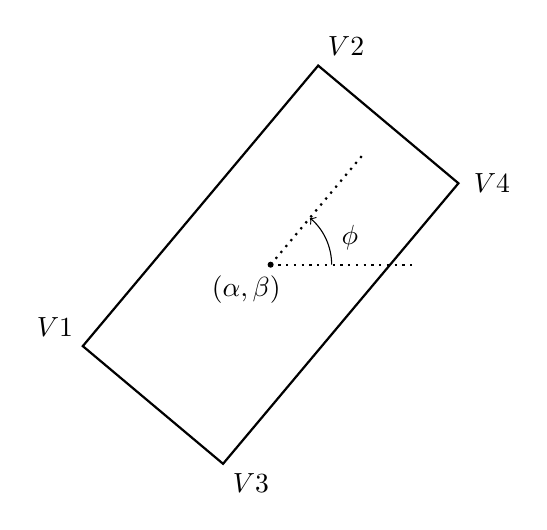
\begin{tikzpicture}[scale=1.55]

% Parameters (arbitrary for illustration)
\def\ll{3}
\def\ww{1.5}
\def\alphaa{-0.5}
\def\betaa{-0.5}
\def\phii{50}

% Derived quantities
\pgfmathsetmacro{\phirad}{\phii * pi / 180}
\pgfmathsetmacro{\hll}{\ll/2}
\pgfmathsetmacro{\hww}{\ww/2}
\pgfmathsetmacro{\ux}{cos(\phii)}
\pgfmathsetmacro{\uy}{sin(\phii)}
\pgfmathsetmacro{\vx}{-sin(\phii)}
\pgfmathsetmacro{\vy}{cos(\phii)}

% Rectangle vertices
\coordinate (V1) at ({\alphaa - \hll*\ux + \hww*\vx}, {\betaa - \hll*\uy + \hww*\vy});
\coordinate (V2) at ({\alphaa + \hll*\ux + \hww*\vx}, {\betaa + \hll*\uy + \hww*\vy});
\coordinate (V4) at ({\alphaa + \hll*\ux - \hww*\vx}, {\betaa + \hll*\uy - \hww*\vy});
\coordinate (V3) at ({\alphaa - \hll*\ux - \hww*\vx}, {\betaa - \hll*\uy - \hww*\vy});

% Draw rectangle
\draw[thick] (V1) -- (V2) -- (V4) -- (V3) -- cycle;

% Draw the black point
\filldraw[black] (\alphaa,\betaa) circle (0.02);

% Add text label near the point
\node at ({\alphaa - 0.2}, {\betaa - 0.2}) {$(\alpha, \beta)$};

% Reference lines for inclination angle
\draw[thick, dotted] (\alphaa,\betaa) -- ++(1.2,0); % x-axis reference
\draw[thick, dotted] (\alphaa,\betaa) -- ++({1.2*cos(\phii)}, {1.2*sin(\phii)}); % inclined direction

% Inclination angle arc and label (slightly lifted)
\draw[->] (\alphaa,\betaa) ++(0:0.5) arc[start angle=0, end angle=\phii, radius=0.5];
\node at ({\alphaa + 0.65*cos(\phirad/2)}, {\betaa + 0.7*sin(\phirad/2) + 0.22}) {$\phi$};

% Vertex labels
\node[above left]  at (V1) {$V1$};
\node[above right] at (V2) {$V2$};
\node[below right] at (V3) {$V3$};
\node[right=2pt] at (V4) {$V4$};

\end{tikzpicture}
\end{center}
\newline
$V1V2$ or $V3V4$ and $V1V3$ or $V2V4$ are the respective sides that represent the length and the width of the rectangle.
\newline
In order to determine the coordinates of the vertices, we begin with the following step. From the known parameters, we first calculate the midpoint coordinates of both the shorter sides (widths). Let us denote midpoint of $V1V3$ as $M$ and midpoint of $V2V4$ as $N$. By simple trigonometry, we can observe the following - 

$$M_x = \alpha-(l/2)*\cos\phi$$

$$M_y = \beta-(l/2)*\sin\phi$$

$$N_x = \alpha+(l/2)*\cos\phi$$

$$N_y = \beta+(l/2)*\sin\phi$$
\newline
where $A_x$ and $A_y$ are the X and Y coordinates of point $A$. The following diagram shows the location of M and N as well.
\begin{center}
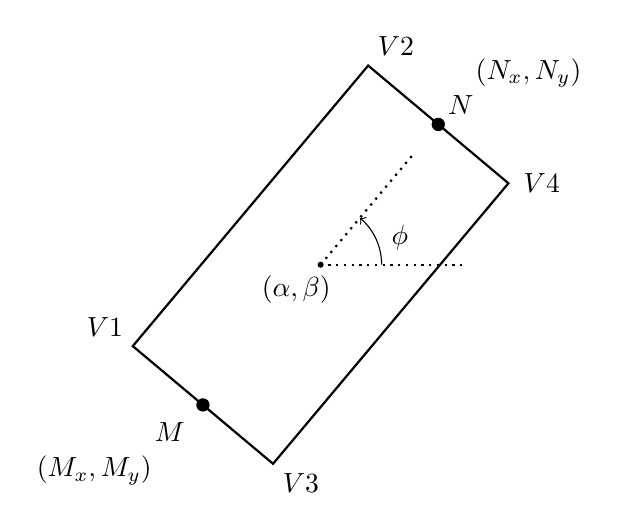
\begin{tikzpicture}[scale=1.55]

% Parameters (arbitrary for illustration)
\def\ll{3}
\def\ww{1.5}
\def\alphaa{-0.5}
\def\betaa{-0.5}
\def\phii{50}

% Derived quantities
\pgfmathsetmacro{\phirad}{\phii * pi / 180}
\pgfmathsetmacro{\hll}{\ll/2}
\pgfmathsetmacro{\hww}{\ww/2}
\pgfmathsetmacro{\ux}{cos(\phii)}
\pgfmathsetmacro{\uy}{sin(\phii)}
\pgfmathsetmacro{\vx}{-sin(\phii)}
\pgfmathsetmacro{\vy}{cos(\phii)}

% Rectangle vertices
\coordinate (V1) at ({\alphaa - \hll*\ux + \hww*\vx}, {\betaa - \hll*\uy + \hww*\vy});
\coordinate (V2) at ({\alphaa + \hll*\ux + \hww*\vx}, {\betaa + \hll*\uy + \hww*\vy});
\coordinate (V4) at ({\alphaa + \hll*\ux - \hww*\vx}, {\betaa + \hll*\uy - \hww*\vy});
\coordinate (V3) at ({\alphaa - \hll*\ux - \hww*\vx}, {\betaa - \hll*\uy - \hww*\vy});

% Draw rectangle
\draw[thick] (V1) -- (V2) -- (V4) -- (V3) -- cycle;

% Draw the black point
\filldraw[black] (\alphaa,\betaa) circle (0.02);

% Add text label near the point
\node at ({\alphaa - 0.2}, {\betaa - 0.2}) {$(\alpha, \beta)$};

% Reference lines for inclination angle
\draw[thick, dotted] (\alphaa,\betaa) -- ++(1.2,0); % x-axis reference
\draw[thick, dotted] (\alphaa,\betaa) -- ++({1.2*cos(\phii)}, {1.2*sin(\phii)}); % inclined direction

% Inclination angle arc and label (slightly lifted)
\draw[->] (\alphaa,\betaa) ++(0:0.5) arc[start angle=0, end angle=\phii, radius=0.5];
\node at ({\alphaa + 0.65*cos(\phirad/2)}, {\betaa + 0.7*sin(\phirad/2) + 0.22}) {$\phi$};
% Vertex labels
\node[above left]  at (V1) {$V1$};
\node[above right] at (V2) {$V2$};
\node[below right] at (V3) {$V3$};
\node[right=2pt] at (V4) {$V4$};

% Midpoints M and N based on given formulas
\pgfmathsetmacro{\Mx}{\alphaa - \hll * \ux}
\pgfmathsetmacro{\My}{\betaa - \hll * \uy}
\pgfmathsetmacro{\Nx}{\alphaa + \hll * \ux}
\pgfmathsetmacro{\Ny}{\betaa + \hll * \uy}

% Plot M and N
\filldraw[black] (\Mx,\My) circle (0.1/2);
\node[below left=3pt] at (\Mx,\My) {$M$};
\node[below left=15pt] at (\Mx,\My) {$(M_x, M_y)$};

\filldraw[black] (\Nx,\Ny) circle (0.1/2);
\node[above right] at (\Nx,\Ny) {$N$};
\node[above right=10pt] at (\Nx,\Ny) {$(N_x, N_y)$};
\end{tikzpicture}
\end{center}
\newline
We can again use simple trigonometry to obtain the coordinates of all the 4 vertices, since we now know the midpoints of the widths.
%\clearpage
The coordinates of the 4 vertices are obtained as follows - 

\[
\begin{aligned}
V1_x &= M_x - \frac{w}{2} \sin\phi, \quad &V1_y &= M_y + \frac{w}{2} \cos\phi \\[6pt]
V2_x &= N_x - \frac{w}{2} \sin\phi, \quad &V2_y &= N_y + \frac{w}{2} \cos\phi \\[6pt]
V3_x &= M_x + \frac{w}{2} \sin\phi, \quad &V3_y &= M_y - \frac{w}{2} \cos\phi \\[6pt]
V4_x &= N_x + \frac{w}{2} \sin\phi, \quad &V4_y &= N_y - \frac{w}{2} \cos\phi
\end{aligned}
\]
\newline
where $A_x$ and $A_y$ are the X and Y coordinates of point $A$.
This is how the obstacle is being defined as a rectangular object. We shall now move on to see how the links of the robot are defined.
\subsection{Defining the First link}
Once we have the obstacle, we can move onto defining the first link of the robot as a simple rod hinged at one end, about the origin of the coordinate system, and having length 3 units. So, the first link can basically describe a circle of radius 3 units, centered at the origin. For computation purposes, we choose the rectangle parameters in such a way that the obstacle is completely or partially inside this circle. The following diagram shows the construction of the first link, and the circle described by it. 


\begin{center}
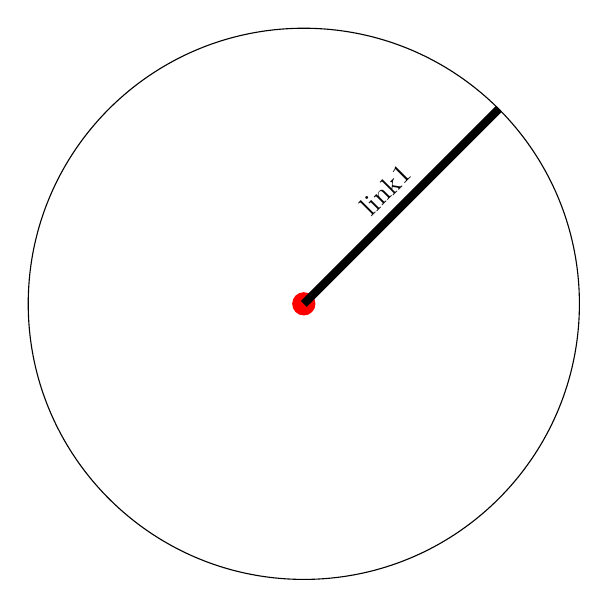
\begin{tikzpicture}
  % Draw circle with radius 3.5
  \draw (0,0) circle (3.5);

  % Draw center dot in red with radius 4pt
  \filldraw[red] (0,0) circle (4pt);

  % Draw radius line with annotation "link1" on the line
  \draw[line width=3pt] (0,0) -- (2.475, 2.475) node[pos=0.5, above, sloped] {link1};

\end{tikzpicture}
\end{center}
We can now place the obstacle fully or partially inside this circle, by choosing appropriate parameters for the rectangle. Note that we shall not place the obstacle in ways that overlap with the origin, because in such cases we cannot construct the first link and it is a collision by default.

\begin{center}
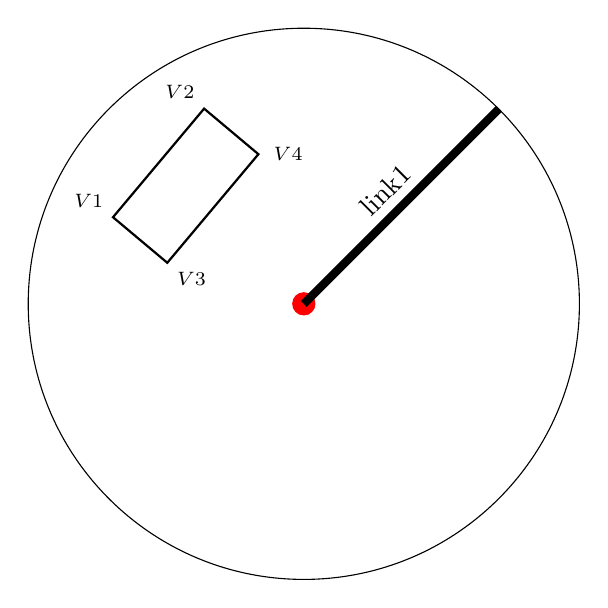
\begin{tikzpicture}
  % Draw circle with radius 3.5
  \draw (0,0) circle (3.5);

  % Draw center dot in red with radius 4pt
  \filldraw[red] (0,0) circle (4pt);

  % Draw radius line with annotation "link1" on the line
  \draw[line width=3pt] (0,0) -- (2.475, 2.475) node[pos=0.5, above, sloped] {link1};

  % Scale and shift obstacle inside circle (more left and up)
  \begin{scope}[scale=0.6, shift={(-2.0,3*1.0)}]  
    % Parameters (arbitrary for illustration)
    \def\ll{3}
    \def\ww{1.5}
    \def\alphaa{-0.5}
    \def\betaa{-0.5}
    \def\phii{50}

    % Derived quantities
    \pgfmathsetmacro{\phirad}{\phii * pi / 180}
    \pgfmathsetmacro{\hll}{\ll/2}
    \pgfmathsetmacro{\hww}{\ww/2}
    \pgfmathsetmacro{\ux}{cos(\phii)}
    \pgfmathsetmacro{\uy}{sin(\phii)}
    \pgfmathsetmacro{\vx}{-sin(\phii)}
    \pgfmathsetmacro{\vy}{cos(\phii)}

    % Rectangle vertices
    \coordinate (V1) at ({\alphaa - \hll*\ux + \hww*\vx}, {\betaa - \hll*\uy + \hww*\vy});
    \coordinate (V2) at ({\alphaa + \hll*\ux + \hww*\vx}, {\betaa + \hll*\uy + \hww*\vy});
    \coordinate (V4) at ({\alphaa + \hll*\ux - \hww*\vx}, {\betaa + \hll*\uy - \hww*\vy});
    \coordinate (V3) at ({\alphaa - \hll*\ux - \hww*\vx}, {\betaa - \hll*\uy - \hww*\vy});

    % Draw rectangle
    \draw[thick] (V1) -- (V2) -- (V4) -- (V3) -- cycle;

    % Draw the black point
    %\filldraw[black] (\alphaa,\betaa) circle (0.02);

    % Add text label near the point
    %\node at ({\alphaa - 0.2}, {\betaa - 0.2}) {$(\alpha, \beta)$};

    % Reference lines for inclination angle
    %\draw[thick, dotted] (\alphaa,\betaa) -- ++(1.2,0); % x-axis reference
    %\draw[thick, dotted] (\alphaa,\betaa) -- ++({1.2*cos(\phii)}, {1.2*sin(\phii)}); % inclined direction

    % Inclination angle arc and label (slightly lifted)
    %\draw[->] (\alphaa,\betaa) ++(0:0.5) arc[start angle=0, end angle=\phii, radius=0.5];
    %\node at ({\alphaa + 0.65*cos(\phirad/2)}, {\betaa + 0.7*sin(\phirad/2) + 0.22}) {$\phi$};

    % Vertex labels with smaller font
    \node[above left]  at (V1) {\scriptsize $V1$};
    \node[above left] at (V2) {\scriptsize $V2$};
    \node[below right] at (V3) {\scriptsize $V3$};
    \node[right=2pt]   at (V4) {\scriptsize $V4$};

  \end{scope}

\end{tikzpicture}
\end{center}
By seeing, we can easily observe that vertices $V_3$ and $V_4$ are the points where the first link will collide when it tries to rotate a full 360 degrees, in both directions. So now we try and come up with an algorithm that gives us the 2 collision points on the rectangle, and essentially the safe operating range of $\theta_1$ (angle rotated by the first link)
\clearpage
\subsection{Determining the Collision limits for the First link}
\underline{\textbf{Algorithm used to detect the collision limits for link 1:}}
\newline
\newline
There can be 5 broad way of classifying how the obstacle is placed within/near the circle as follows - 
\newline
Case 1: Obstacle is completely inside the circle
\newline
Case 2: Obstacle has just 1 vertex outside the circle
\newline
Case 3: Obstacle has 2 vertices outside the circle
\newline
Case 4: Obstacle has 3 vertices outside the circle
\newline
Case 5: Obstacle has all of its 4 vertices outside the circle
\newline
For the purpose of analysis of the first link, we are not considering obstacles completely outside the circle, nor do we place the obstacle in configurations intersecting the origin, as mentioned before. We can now see the idea that is used to deal with the above 5 cases, and the algorithm that incorporates all the cases.
\newline
\newline
\underline{\textbf{Case 1:}}
\newline
This is the most simplest case, wherein the obstacle completely lies within the circle described by the first link. The obstacle can have any orientation, position and dimensions. So our algorithm must be able to find the collision limits for every feasible configuration satisfying this case. The following diagram shows the collision limits that we are required to determine. We basically have to compute the range of $\theta_1$ for which there will be collision (remaining range is collision-free motion).
\begin{center}
\scalebox{.9}{ % Uniform scaling of everything
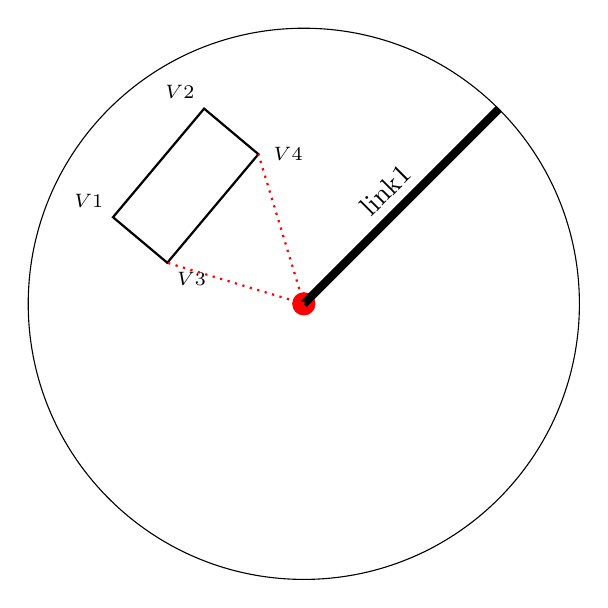
\begin{tikzpicture}
  % Draw circle with radius 3.5
  \draw (0,0) circle (3.5);

  % Draw center dot in red with radius 4pt
  \filldraw[red] (0,0) circle (4pt);

  % Draw radius line with annotation "link1" on the line
  \draw[line width=3pt] (0,0) -- (2.475, 2.475) node[pos=0.5, above, sloped] {link1};

  % --- Scope for obstacle (scaled and shifted)
  \begin{scope}[scale=0.6, shift={(-2.0,3.0)}]  
    \def\ll{3}
    \def\ww{1.5}
    \def\alphaa{-0.5}
    \def\betaa{-0.5}
    \def\phii{50}

    \pgfmathsetmacro{\phirad}{\phii * pi / 180}
    \pgfmathsetmacro{\hll}{\ll/2}
    \pgfmathsetmacro{\hww}{\ww/2}
    \pgfmathsetmacro{\ux}{cos(\phii)}
    \pgfmathsetmacro{\uy}{sin(\phii)}
    \pgfmathsetmacro{\vx}{-sin(\phii)}
    \pgfmathsetmacro{\vy}{cos(\phii)}

    \coordinate (V1) at ({\alphaa - \hll*\ux + \hww*\vx}, {\betaa - \hll*\uy + \hww*\vy});
    \coordinate (V2) at ({\alphaa + \hll*\ux + \hww*\vx}, {\betaa + \hll*\uy + \hww*\vy});
    \coordinate (V4) at ({\alphaa + \hll*\ux - \hww*\vx}, {\betaa + \hll*\uy - \hww*\vy});
    \coordinate (V3) at ({\alphaa - \hll*\ux - \hww*\vx}, {\betaa - \hll*\uy - \hww*\vy});

    % Draw rectangle
    \draw[thick] (V1) -- (V2) -- (V4) -- (V3) -- cycle;

    % Labels
    \node[above left]  at (V1) {\scriptsize $V1$};
    \node[above left]  at (V2) {\scriptsize $V2$};
    \node[below right] at (V3) {\scriptsize $V3$};
    \node[right=2pt]   at (V4) {\scriptsize $V4$};

    % Save transformed V3 and V4 positions globally
    \coordinate (GLOBV3) at (V3);
    \coordinate (GLOBV4) at (V4);
  \end{scope}

  % --- Red dotted radii from origin to V3 and V4 (outside scope!)
  \draw[red, dotted, thick] (0,0) -- (GLOBV3);
  \draw[red, dotted, thick] (0,0) -- (GLOBV4);
\end{tikzpicture}
}
\end{center}
\clearpage
\underline{\textbf{The Algorithm:}}
\newline
We start off by calculating the angle between the positive X-Axis and the line segment joining the origin and vertex, for each of the 4 vertices.
\newline
Let's say the coordinate of a vertex is ($V_x$, $V_y$), so the corresponding angle between the positive X-Axis and the line segment joining the origin and this vertex is given by the following equation - $$\gamma = \tan^{-1}{(\frac{V_y}{V_x})}$$
\newline
We know that the range of the tan inverse function is from $-\pi$ to $\pi$. Hence we normalize this to $0$ to $2\pi$. So now we know the angles corresponding to all the 4 vertices of the obstacle, lying between 0 and 360 degrees. Let these angles be $\gamma_1, \gamma_2, \gamma_3$, and$ \gamma_4$.
\newline
We now select any 2 of these angles, in all possible combinations. After selecting 2 angles, we compute their absolute difference. Since we have 4 angles, we end up with 6 pair wise differences as follows:
$\gamma_1 - \gamma_2$, $\gamma_1 - \gamma_3$, $\gamma_1 - \gamma_4$, $\gamma_2 - \gamma_3$, $\gamma_2 - \gamma_4$, and 
$\gamma_3 - \gamma_4$.
Whichever difference is maximum, those 2 vertices corresonding to that pair shall give us the collision limits. Note that we only need the absolute value of the difference, so the sign does not matter. In our case, $\gamma_3 - \gamma_4$ turns out to be the maximum of all the 6 pair wise differences. So the vertices $V3$ and $V4$ become the collision limits for link 1.
\newline
\newline
\underline{\textbf{Case 2:}}
\newline
In this case, we have exactly one of the vertices of the obstacle to lie outside the circle. This case turns out be be very similar to the first case. We use the exact same algorithm to find out the collision limits. One thing we do differently here is that we exclude the vertex that lies outside the cirlce. So the pair wise differences are only taken between the remaining 3 vertices which are inside, and that pair is chosen which yields maximum difference. From here, we can get the collision limits for link 1 in the same manner. 
\newline
\newline
In order to determine whether a vertex lies inside or outside the circle, we can simply use the equation of circle to check with the points.
\newline
This is the equation of our circle: $x^2 + y^2 = 3^2$, as the radius is the link length, which is 3 units.
So bringing all terms to one side, we get
%\newline
$S$ as $x^2 + y^2 - 9 = 0$
\newline
We can now substitute the coordinates of each vertex into $S$.
\newline
If $S>$0, point lies outside the cirle, and if $S<$0, point lies inside the circle.
\newline
where $S =x^2 + y^2 - 9 $
\newline
In the next few cases,this circle equation becomes very useful to check whether the vertices lie inside or outside the circle. Even for the first case, the condition $S<$0 would have been satsfied by every point, which means that every point is inside the circle.
\newline
\newline
\underline{\textbf{Case 3:}}
\newline
In this case, we have 2 of the vertices of the obstacle to lie outside the circle. First we calculate the value of $S$, which is equal to $x^2 + y^2 - 9$, for all the 4 vertices, and throw those vertices for which $S>$0. We basically ignore the vertices which are lying outside the circle, as these don't help in finding the collision limits.
\newline
\newline
It has been observed that in this case, we can further make classifications on how the obstacle can be configured. The first subcase is similar to what we have done till now, where the collision limits are given by the vertices subtending the maximum angular span. However, the second subcase talks about the following configuration, where the one of the collision limit is one of the in-lying vertices, and the other collision limit is one of the intersection points of the obstacle and circle.
\newline
\newline
The following 2 figures will help us understand these 2 subcases which were mentioned above.
\begin{figure}[h!]
    \centering
    \begin{minipage}{0.48\textwidth}
        \centering
        \includegraphics[width=\linewidth]{C-Space_series/c2s1.png}
        \caption{Collision limits are \newline
        determined from vertices as usual}
        \label{fig:c2s1}
    \end{minipage}
    \hfill
    \begin{minipage}{0.48\textwidth}
        \centering
        \includegraphics[width=\linewidth]{n.png}
        \caption{Collision limits depend on one vertex and one intersection point}
        \label{fig:n}
    \end{minipage}
\end{figure}
\newline
\underline{\textbf{The Algorithm:}}
\newline
We start off by eliminating those vertices which are outside the circle by using the circle equation given by $S$.
\newline
$$S>0$$The above inequality implies that the point is thrown from further analysis.
\newline
We then calculate the 2 intersection points of the circle and the rectangle, by using the circle equation $S$ and sampling points on the edges of the rectangle. We would be checking which of these sampled points satisfy the equation $S=$0. Let us call these intersection points as $M_1$ and $M_2$. We now have 2 intersection points and 2 in-lying vertices. Let $P$ be a list containing these 4 points, where $P_i$ denotes the \textit{i}-th
 element of the following list.
$$P=[M_1, M_2, V_q, V_r]$$
where $V_q$ and $V_r$ are the in-lying vertices, or the vertices that remain after throwing the out-lying vertices.
From here, the process is similar to what we have been doing in the first few cases. We compute the angle between the positive X-Axis and the line segment joining the origin and $P_i$, for all the 4 points of the list. These angles are calculated by using the same tan inverse formula, and normalized to the range of 0 to 360 degrees. Once we have the 4 angles, we compute all the pair wise differences and select the pair which yields maximum absolute difference. These 2 points obtained shall give us the collision limits. Note that the collision limits maybe 2 vertices, or a vertex and an intersection point, depending on how the obstacle is configured. Given below are 2 more examples coming under this case.
\begin{figure}[h!]
    \centering
    \begin{minipage}{0.44\textwidth}
        \centering
        \includegraphics[width=\linewidth]{C-Space_series/n6.png}
        \caption{Ex.1}
        \label{fig:n6}
    \end{minipage}
    \hfill
    \begin{minipage}{0.44\textwidth}
        \centering
        \includegraphics[width=\linewidth]{C-Space_series/n3.png}
        \caption{Ex.2}
        \label{fig:n3}
    \end{minipage}
\end{figure}
\newline
\underline{\textbf{Case 4:}}
\newline
In this case, we have 3 vertices of the obstacle to lie outside the circle. As we have done before, we calculate the value of $S$, which is equal to $x^2 + y^2 - 9$, for all the 4 vertices, and throw the 3 vertices for which $S>$0.
\newline
\newline
Since 3 vertices are outside the cirlce, it obviously means that there is only 1 vertex inside the circle, and that there are again 2 intersection points. The following figures represent configurations of the obstacle satisfying this case.
\begin{figure}[h!]
    \centering
    \begin{minipage}{0.48\textwidth}
        \centering
        \includegraphics[width=\linewidth]{C-Space_series/n8.png}
        \caption{Ex.1}
        \label{fig:n8}
    \end{minipage}
    \hfill
    \begin{minipage}{0.48\textwidth}
        \centering
        \includegraphics[width=\linewidth]{C-Space_series/n10.png}
        \caption{Ex.2}
        \label{fig:n10}
    \end{minipage}
\end{figure}
\newline
We repeat the same process that we have done in previous case.
We just have to calculate the intersection points, and store them in a list along with that 1 in-lying vertex; now for these 3 points in the list, we calculate the pair wise differences of the angles and pick the pair which again yields the maximum absolute difference.
\newline
\newline
\underline{\textbf{Case 5:}}
\newline
In this case, we have all the vertices of the obstacle to lie outside the circle. By seeing a few figures, we can directly observe that the 2 intersection points of the rectangle and circle will also be the 2 collision limits for the first link. We have to make sure that $S>$0 for all the vertices, and then compute the intersection points $M_1$ and $M_2$ by sampling points on the rectangle edges and checking which of those are satisfying the equation of circle $S$=0. We can observe a few examples in the next page.
\clearpage
\begin{figure}[h!]
    \centering
    \begin{minipage}{0.48\textwidth}
        \centering
        \includegraphics[width=\linewidth]{C-Space_series/a1.png}
        \caption{Ex.1}
        \label{fig:a1}
    \end{minipage}
    \hfill
    \begin{minipage}{0.48\textwidth}
        \centering
        \includegraphics[width=\linewidth]{C-Space_series/a2.png}
        \caption{Ex.2}
        \label{fig:a2}
    \end{minipage}
\end{figure}
Once we have the intersection points $M_1$ and $M_2$, these 2 points directly become the collision limits, and we can calculate the angles corresponding to these points from the tan inverse formula as we have done for all other cases.
\newline
\newline
\underline{\textbf{Final Algorithm to handle all 5 cases:}}
\newline
\begin{itemize}
    \item Make a list $V$ containing all the vertices of the rectangle. Let $V_i$ be the $i$-th element of this list.
    
    \item Compute the value of the distance $OV_i$ for all points in $V$, where $O$ is the origin. Let R denote the radius of the circle, which is 3 units.
    
    \item Make a new list $B$, and append all the computed $OV_i$ values to it. Now, the $j$-th element of list $B$ shall be represented as $B_j$.
    
    \item Use the following conditionals to decide the case:
    \begin{itemize}
        \renewcommand\labelitemi{--}
        \item If all elements of $B < R$, use case 1.
        \item If only one element of $B > R$, use case 2.
        \item If two elements of $B > R$, use case 3.
        \item If three elements of $B > R$, use case 4.
        \item If all elements of $B > R$, use case 5.
    \end{itemize}
    
    \item In code, cases 1 and 2 will be combined as "if condition" 1, and cases 3,4 and 5 are combined as "if condition" 2, due to similarities.
\end{itemize}
\clearpage
\subsection{Defining the Second link}
The second link will be dimensionally identical to the first link. The start of the second link is connected to the end of the first link, by a revolute joint. Obviously, even the first link is connected to the base via a revolute joint. That is why we call this as a 2R robot, meaning there are 2 revolute pairs. The following figure shows the construction of the second link, attached to the first.
\begin{center}
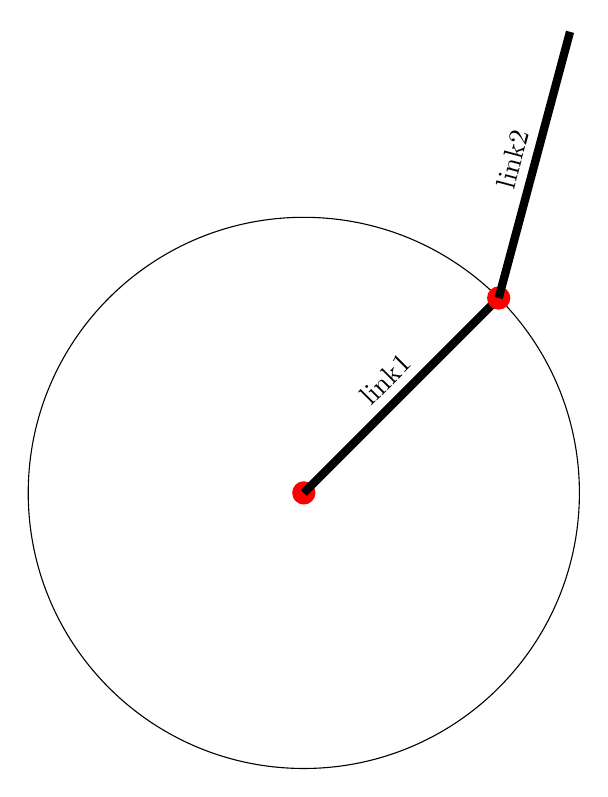
\begin{tikzpicture}
  % Draw circle with radius 3.5
  \draw (0,0) circle (3.5);

  % Draw center dot in red with radius 4pt
  \filldraw[red] (0,0) circle (4pt);

  % First link (link1): 45 degrees from center
  \pgfmathsetmacro{\r}{3.5}
  \pgfmathsetmacro{\xone}{\r * cos(45)}
  \pgfmathsetmacro{\yone}{\r * sin(45)}
  \coordinate (P1) at (\xone,\yone);
  \draw[line width=3pt] (0,0) -- (P1) node[pos=0.5, above, sloped] {link1};
  \filldraw[red] (P1) circle (4pt);

  % Second link (link2): 75 degrees from x-axis (i.e., 30° from link1)
  \pgfmathsetmacro{\angleTwo}{75}
  \pgfmathsetmacro{\xTwo}{\xone + \r * cos(\angleTwo)}
  \pgfmathsetmacro{\yTwo}{\yone + \r * sin(\angleTwo)}
  \coordinate (P2) at (\xTwo,\yTwo);
  \draw[line width=3pt] (P1) -- (P2) node[pos=0.5, above, sloped] {link2};

\end{tikzpicture}
\end{center}
For the purpose of geometric analysis, we aren't taking into account any joint rotation limits, meaning that both $\theta_1$ and $\theta_2$ can take any value between 0 and 360 degrees. $\theta_1$ is measured from the positive X-Axis in Anticlockwise direction, whereas $\theta_2$ is measured from the direction of the first link. We can later define how $\theta_2$ is exactly defined. Somtimes we may prefer the acute angle between link 1 and link 2, sometimes the obtuse angle. During computation, we have to clearly define $\theta_2$. In code, $\theta_2$ is taken as the acute angle between link 1 and link 2.
\clearpage
\subsection{Obtaining range of joint angles for safe operation}
\subsubsection{Complete safe operating range of $\theta_1$}
For a given position of the obstacle, we will have to obtain the full ranges of both $\theta_1$ and $\theta_2$ for which there will be a collision-free motion. We have already identified the collision limits for link 1 alone, without considering the second link, but certain configurations of the 2R robot in which the the first link isn't colliding with the obstacle may still lead to collision due to the presence of the second link, in certain orientations.
\newline
\newline
We shall proceed in the following manner - we will try to compute a safe operating range of $\theta_1$ for which $\theta_2$ can take any value, meaning that this range of $\theta_1$ is completely safe independent of the value of $\theta_2$. We then move onto the remaining range of $\theta_1$ and obtain the ranges of $\theta_2$ which cause collision. Note that we will not go into the collision regions of $\theta_1$, as these configurations will always have the first link hitting the obstacle irrespective of thet value of $\theta_2$. We have already done this analysis in the previous sub-section.
\newline
\newline
The figures presented below correspond to the preceding discussion.
\begin{figure}[h!]
    \centering
    \begin{minipage}{0.49\textwidth}
        \centering
        \includegraphics[width=\linewidth]{C-Space_series/b1.png}
        \caption{Ex.1}
        \label{fig:b1}
    \end{minipage}
    \hfill
    \begin{minipage}{0.49\textwidth}
        \centering
        \includegraphics[width=\linewidth]{C-Space_series/b2.png}
        \caption{Ex.2}
        \label{fig:a2}
    \end{minipage}
\end{figure}
\newline
The 2 figures above show the collision limits for the first link, as denoted by the red dotted-radii. The (blue/magenta) segment from the origin to the circumference of the circle is the first link, and the segment which starts from the point where the first link ends, is the the second link. More details of these figures are explained in the next page.
\newline
\newline
\newline
Let's take the figure on the left, for an example. We know that the red dotted-radii is the collision range corresponding to link 1. In order to find the complete safe range of $\theta_1$ for which the robot never collides with the obstacle irrespective of the value of $\theta_2$, we make constructions in the following manner - 
\newline
\begin{itemize}
  \item Take any of the collision limit points as the starting point — let's say the right vertex \( V_4 \).
  
  \item From this point, construct a line segment of length 3 units such that it perfectly ends on the circumference of the existing circle.
  
  \item This newly drawn segment represents the second link of the robot.
  
  \item Now, construct the radius (first link) from the origin to this point on the circle.
  
  \item The configuration attained now corresponds to the extreme value of \( \theta_1 \) that the robot can take to ensure safe operation.
  
  \item Since this is a limiting case, we assume the second link just grazes the vertex \( V_4 \), which is why we constructed the second link directly from \( V_4 \).
  
  \item We observe that if \( \theta_1 \) is increased even slightly beyond this angle, the second link can no longer rotate freely through \( 360^\circ \).
  
  \item In such a case, there exists both an upper and a lower limit for \( \theta_2 \) as well.
  
  \item The upper limit of \( \theta_2 \) corresponds to the configuration where the second link just grazes the width-containing side \( V_2V_4 \).
  
  \item The lower limit of \( \theta_2 \) corresponds to the configuration where the second link just grazes the length-containing side \( V_3V_4 \).
  
  \item What we aim to do here is to find the range of \( \theta_2 \) for which there will be a collision with the obstacle, given a certain deviation of \( \theta_1 \) from its safe limit.
  
  \item Note that this safe limit for \( \theta_1 \) is the one obtained by drawing a 3 unit long segment from $V4$ that ends exactly on the circle, and constructing the radius to that point. It is not the collision limits of $\theta_1$ that are represented by the red dotted-radii. The mathematical calculations are shown below.
\end{itemize}
Let us denote the coordinate of the vertex $V4$ as simply $(V_x, V_y)$. In our case, it happens to be V4, in other cases the point maybe a different vertex or an intersetion. That is why we aren't taking the coordinates with subsript 4.
We can take the coordinates of any point lying on the cirumference of the circle as follows - $$(x,y)=(R\cos\theta, R\sin\theta)$$, where $R$ is the radius of the circle and $\theta$ is the argument of that point in parametric form.
\newline
\newline
Now we use the simple distance formula between this point on the circle and vertex $(V_x, V_y)$. We know that the second link is also 3 units long, so this distance equals 3.
$$(V_x-R\cos\theta)^2 + (V_y-R\sin\theta)^2=3^2$$
The above equation uses the simple distance formula between 2 points. We can also substitute R as 3, since the radius of the circle is also 3 units. So the equation now becomes - $$(V_x-3\cos\theta)^2 + (V_y-3\sin\theta)^2=9$$
It can be simplified as follows - 
$$(V_x^2 + 9\cos^2\theta-6V_x\cos\theta)+(V_y^2 + 9\sin^2\theta-6V_y\sin\theta)=9$$
$$V_x^2 + V_y^2 = 6V_x\cos\theta+6V_y\sin\theta$$
We then take - 
\[
A = V_x, \quad B = V_y, \quad C = \frac{V_x^2 + V_y^2}{6}
\]
We finally get - 
\[
A\cos\theta + B\sin\theta = C
\]
\clearpage
The equation $A\cos\theta + B\sin\theta = C$ can be solved using the auxiliary angle method as follows - 

We are given the equation:
\[
A\cos\theta + B\sin\theta = C
\]

Define $W$ and $\alpha$ as follows - 
\[
W = \sqrt{A^2 + B^2}, \quad \alpha = \tan^{-1}\left(\frac{B}{A}\right)
\]

Then we rewrite the left-hand side as:
\[
A\cos\theta + B\sin\theta = W\cos(\theta - \alpha)
\]

So the equation becomes:
\[
W\cos(\theta - \alpha) = C
\]

Which implies:
\[
\cos(\theta - \alpha) = \frac{C}{W}
\]

This equation has real solutions only if:
\[
\left| \frac{C}{W} \right| \leq 1
\]

Therefore, the general solution is:
\[
\theta = \alpha \pm \cos^{-1}\left( \frac{C}{W} \right)
\]

Substituting back for $\alpha$ and $W$, we get:
\[
\theta = \tan^{-1}\left(\frac{B}{A}\right) \pm \cos^{-1}\left(\frac{C}{\sqrt{A^2 + B^2}}\right)
\]
\newline
\newline
From here, we can get 2 angles, which means that there can be 2 points on the circle at a distance of 3 units from vertex $V4$. We only contsider the solution that produces a line segment that doesn't intersect the obstacle.
\newline
We can check for self-intersection in the following manner. If the segment self-intersects, it means that some portion of that segment lies in the collision limit of $\theta_1$. This means that some points on this segment are within the sector enclosed by the collision limits of $\theta_1$.
\newline
We sample a few equally spaced points along the segment and check if any point satisfies the following two conditions:
\begin{itemize}
    \item The distance from the origin to the sampled point is less than the radius: \( OP < R \)
    \item The argument angle of that point lies within the collision limit range of link 1: \( \theta_{\text{min}} \leq \theta \leq \theta_{\text{max}} \)
\end{itemize}
If even a single point of the segment satisfies the conditions above, that segment is rejected.
\newline
\newline
From this analysis, we can determine the configurations that correspond to the complete safe range of \(\theta_1\), for which the robot never collides with the obstacle regardless of the value of \(\theta_2\). The following figures represent a few other obstacle configurations.
\begin{figure}[h!]
    \centering
    \begin{minipage}{0.49\textwidth}
        \centering
        \includegraphics[width=\linewidth]{C-Space_series/c2.png}
        \caption{Ex.1}
        \label{fig:c2}
    \end{minipage}
    \hfill
    \begin{minipage}{0.49\textwidth}
        \centering
        \includegraphics[width=\linewidth]{C-Space_series/c3.png}
        \caption{Ex.2}
        \label{fig:c3}
    \end{minipage}
\end{figure}
\newline
We can easily get the angles corresponding to these points on the circumference from the same tan inverse formula, and normalize it between 0 and 360 degrees.
\clearpage
\subsubsection{Collision range of $\theta_2$}
Let us start off with the below example, which was used for the previous sub-case as well.
\begin{figure}[h!]
    \centering
    \begin{minipage}{0.8\textwidth}
        \centering
        \includegraphics[width=\linewidth]{C-Space_series/b1.png}
        \caption{Figure depicts the 2 extreme configurations of the robot for which there is no collision at all}
        \label{fig:b1}
    \end{minipage}
    \hfill
    
\end{figure}
\newline
The blue and magenta radii indicate the extreme orientations of link 1. In between these 2 extreme radii, we can take any radii as link 1, and the arm will never collide with the obstacle irrespective of the value of $\theta_2$.
\newline
\newline
Only at these extreme orientations of link 1, the end of the second link would just meet the vertex of the obstacle; so we can understand that if we choose any radii which is outside this limit as link 1, there will be some values of $\theta_2$ which will lead to collision.
\newline
\newline
In this section, our goal is to find out the range of $\theta_2$ which results in collision, given we know how much we deviate from the limit, for link 1. This is illustrated in the following figure.
\clearpage
\begin{figure}[h!]
    \centering
    \begin{minipage}{0.8\textwidth}
        \centering
        \includegraphics[width=\linewidth]{C-Space_series/c4.png}
        \caption{Collision range for link 2 in magenta}
        \label{fig:c4}
    \end{minipage}
    \hfill
    
\end{figure}
\newline
\begin{itemize}
    \item Here, we can observe 2 black radii that are drawn. The radii to $P$ denotes the initial configuration of link 1 (one of the safe limits), which is calculated from previous analyses; so the black radii to $P$ here is same as the magenta radii in the previous figure (Figure 14).
    
    \item From this point $P$, we rotate link 1 by some angle dw, to reach point $P_2$ as shown. Now if we try to construct the second link from $P_2$, we can see that it will have an upper and lower limit within which it will collide with the obstacle. The upper limit occurs when link 2 just grazes the width-containing side of the obstacle, and the lower limit occurs when link 2 just grazes the length-contaning side of the obstacle. We have to determine this angle range for $\theta_2$. Once we have this, we will get to know the safe operating regions of $\theta_2$.

    \item The method to find collision points is similar to before. Knowing the coordinates of $P_2$ (after rotating from P) and that link 2 has a length of 3 units, we determine where it collides with the rectangle. The detailed calculations for the collision limits of $\theta_2$ are discussed on the next page.
    
    \item We know point \(P\) from the previous analysis and take its coordinates to be \((P_x, P_y)\), where both \(P_x\) and \(P_y\) are known. The deviation of link 1 from this point will also be known; assume the deviation to be \(dw\). We now know two things — the coordinates of point \(P\) as well as the angular deviation from point \(P\). With this, we calculate the coordinates of point \(P_2\) as follows:
\end{itemize}

\[
P_{2x} = R \cos(dw + \arg(P))
\]
\[
P_{2y} = R \sin(dw + \arg(P))
\]

where:

\[
\begin{array}{l l}
P_{2x}  & \quad \text{--- is the X-coordinate of } P_2 \\
P_{2y}  & \quad \text{--- is the Y-coordinate of } P_2 \\
R       & \quad \text{--- is the radius of the circle} \\
dw      & \quad \text{--- is the deviation from point } P \\
\arg(P) & \quad \text{--- is the argument angle of point } P, \text{ which is given by } \tan^{-1} \left( \frac{P_y}{P_x} \right)
\end{array}
\]

\begin{itemize}
    \item Now, since we have the coordinates of point \(P_2\), we can go ahead with finding the intersection points of link 2 with the obstacle sides.
    
    \item From simple geometry, we can see that link 2 revolves around \(P_2\), with respect to link 1. So the complete range of all configurations of link 2 would be given by the circle centred at \(P_2\), and having radius equal to the length of link 2. Due to the presence of the obstacle, this circle would intersect the rectangle at 2 points, in this case. These 2 intersection points will directly give us the collision limits for \(\theta_2\).
    
    \item We can use the equation of this new circle, say \(S^1\), and sample points on the obstacle edges to check if they satisfy the equation \(S^1 = 0\) or not. Points satisfying \(S^1 = 0\) will give us the 2 points on the obstacle edges.
\end{itemize}

Equation \(S^1\) is as follows:

\[
(x - P_{2x})^2 + (y - P_{2y})^2 = R^2
\]

\clearpage
which simplifies to:

\[
(x - P_{2x})^2 + (y - P_{2y})^2 - 9 = 0
\]

, taking the length of link 2 to be also equal to 3 units.

\end{document}



\end{itemize}
\end{document}

